%%%%%%%%%%%%%%%%%%%%%%%%%%%%%%%%%%%%%%%%%%%%%%%%%%%%%%%%%%%%%%%%%%%%%%%%%%%%%%%
% Memorial para concurso público de Professor Doutor na USP.
%
% Formatação inspirada em:
% * https://tug.org/pracjourn/2008-1/mori/mori.pdf
% * https://github.com/santisoler/phd-thesis
% * https://github.com/compgeolab/dissertation-template
%%%%%%%%%%%%%%%%%%%%%%%%%%%%%%%%%%%%%%%%%%%%%%%%%%%%%%%%%%%%%%%%%%%%%%%%%%%%%%%

%%%%%%%%%%%%%%%%%%%%%%%%%%%%%%%%%%%%%%%%%%%%%%%%%%%%%%%%%%%%%%%%%%%%%%%%%%%%%%%
% Set a class and import packages
\documentclass[10pt,a4paper,oneside]{book}

% Variables
\newcommand{\Year}{2024}
\newcommand{\Author}{Esdras Caleb Oliveira Silva}
\newcommand{\Title}{Memorial e Projeto de Atuação Profissional de \Author{} para concurso público - Professor do Magistério Superior Adjunto-A - IMD/UFRN}
\newcommand{\Email}{esdrascaleb@gmail.com}
\newcommand{\ORCID}{0000-0001-5232-5067}
\newcommand{\GoogleScholar}{zWxct1EAAAAJ}
\newcommand{\Lattes}{5923627359710427}

% Variables for easier typing of some names
\newcommand{\UFF}{Universidade Federal Fluminense}
\newcommand{\UFRN}{Universidade Federal do Rio Grande do Norte}

% Names for citing coauthors
\newcommand{\Me}{\textbf{Uieda, L}}
\newcommand{\Val}{Barbosa, VCF}
\newcommand{\Bi}{Oliveira Jr, VC}
\newcommand{\Paul}{Wessel, P}
\newcommand{\Joaquim}{Luis, J}
\newcommand{\Remko}{Scharroo, R}
\newcommand{\Florian}{Wobbe, F}
\newcommand{\Walter}{Smith, WHF}
\newcommand{\Dongdong}{Tian, D}
\newcommand{\Bridget}{Smith-Konter, B}
\newcommand{\Eric}{Xu, X}
\newcommand{\David}{Sandwell, DT}
\newcommand{\Carla}{Braitenberg, C}
\newcommand{\Naomi}{Ussami, N}
\newcommand{\Manoel}{D'Agrella-Filho, MS}
\newcommand{\JB}{Silva, JBC}
\newcommand{\Dai}{Sales, DP}
\newcommand{\Figura}{Melo, FF}
\newcommand{\Dio}{Carlos, DU}
\newcommand{\BragaVale}{Braga, MA}
\newcommand{\YLi}{Li, Y}
\newcommand{\Angeli}{Angeli, G}
\newcommand{\Peres}{Peres, G}
\newcommand{\Everton}{Bomfim, EP}
\newcommand{\Eder}{Molina, E}
\newcommand{\Gomes}{Gomes, AAS}
\newcommand{\Santiago}{Soler, SR}
\newcommand{\Agustina}{Pesce, A}
\newcommand{\Gimenez}{Gimenez, ME}
\newcommand{\Kristoffer}{Hallam, KAT}
\newcommand{\Guangdong}{Zhao, G}
\newcommand{\Bo}{Chen, B}
\newcommand{\JLiu}{Liu, J}
\newcommand{\LChen}{Chen, L}
\newcommand{\RGuo}{Guo, R}
\newcommand{\MKaban}{Kaban, MK}
\newcommand{\Lindsey}{Heagy, LJ}
\newcommand{\Lion}{Krischer, L}
\newcommand{\Rene}{Gassmoeller, R}
\newcommand{\Bane}{Sullivan, CB}
\newcommand{\Jens}{Klump, JF}
\newcommand{\LBarba}{Barba, LA}
\newcommand{\JBazan}{Bazan, J}
\newcommand{\JBrown}{Brown, J}
\newcommand{\RGuimera}{Guimera, RV}
\newcommand{\MGymrek}{Gymrek, M}
\newcommand{\AHanna}{Alex Hanna}
\newcommand{\KHuff}{Huff, KD}
\newcommand{\DKatz}{Katz, DS}
\newcommand{\CMadan}{Madan, CR}
\newcommand{\KMoerman}{Moerman, KM}
\newcommand{\KNiemeyer}{Niemeyer, KE}
\newcommand{\JPoulson}{Poulson, JL}
\newcommand{\PPrins}{Prins, P}
\newcommand{\KRam}{Ram, K}
\newcommand{\ARokem}{Rokem, A}
\newcommand{\Arfon}{Smith, AM}
\newcommand{\GThiruvathukal}{Thiruvathukal, GK}
\newcommand{\KThyng}{Thyng, KM}
\newcommand{\BWilson}{Wilson, BE}
\newcommand{\Yehudi}{Yehudi, Y}
\newcommand{\Remi}{Rampin, R}
\newcommand{\Hugo}{van Kemenade, H}
\newcommand{\MattTurk}{Turk, M}
\newcommand{\Shapero}{Shapero, D}
\newcommand{\Anderson}{Banihirwe, A}
\newcommand{\Leeman}{Leeman, J}
\newcommand{\JEbbing}{Ebbing, J}
\newcommand{\AGuy}{Guy, A}
\newcommand{\JFarquharson}{Farquharson, J}
\newcommand{\AKushnir}{Kushnir, A}
\newcommand{\FWadsworth}{Wadsworth, F}
\newcommand{\LPerozzi}{Perozzi, L}
\newcommand{\MWieczorek}{Wieczorek, MA}
\newcommand{\LLi}{Li, L}
\newcommand{\Ricardo}{Trindade, RIF}

% Links to webpages I use often
\newcommand{\SantiagoLink}{\href{https://www.santisoler.com/}{Santiago R. Soler}}
\newcommand{\VanderleiLink}{\href{https://www.pinga-lab.org/people/oliveira-jr.html}{Vanderlei C. Oliveira Jr.}}
\newcommand{\SandwellLink}{\href{https://topex.ucsd.edu/sandwell/}{David Sandwell}}
\newcommand{\ValeriaLink}{\href{https://www.pinga-lab.org/people/barbosa.html}{Valéria C. F. Barbosa}}
\newcommand{\PaulLink}{\href{https://www.soest.hawaii.edu/pwessel/}{Paul Wessel}}
\newcommand{\IndiaLink}{\href{https://www.compgeolab.org/team/\#indiauppal}{India Uppal}}
\newcommand{\GelsonLink}{\href{https://www.compgeolab.org/team/\#Souza-junior}{Gelson Ferreira de Souza Junior}}

\newcommand{\GMTLink}{\href{https://www.generic-mapping-tools.org}{Generic Mapping Tools}}
\newcommand{\CompGeoLabLink}{\href{https://www.compgeolab.org/}{Computer-Oriented Geoscience Lab}}
\newcommand{\SwunngLink}{\href{https://softwareunderground.org/}{Software Underground}}
\newcommand{\FatiandoLink}{\href{https://www.fatiando.org}{Fatiando a Terra}}
\newcommand{\PyGMTLink}{\href{https://www.pygmt.org}{PyGMT}}
\newcommand{\SSILink}{\href{https://software.ac.uk/}{Software Sustainability Institute}}

% Import packages
\usepackage[utf8]{inputenc}
\usepackage[T1]{fontenc}
\usepackage[brazil]{babel}
\usepackage{geometry}
\usepackage{graphicx}
\usepackage{amssymb}
\usepackage{amsmath}
\usepackage{mathpazo}
\usepackage{hyperref}
% create fancy headers
\usepackage{fancyhdr}
% commands for managing dates and its formats
\usepackage{datetime2}
% improved urls with proper hyphenation
\usepackage{xurl}
% Control over enumerate and itemize
\usepackage{enumitem}
% Tweak the look of captions
\usepackage{caption}
% To control the style of section titles
\usepackage{titlesec}
% Add the bibliography to the table of contents
\usepackage[nottoc,chapter]{tocbibind}
\usepackage[round,authoryear,sort]{natbib}
% show dois as links on references
\usepackage{doi}
% Icon and fonts (requires using xelatex or luatex)
\usepackage{fontawesome5}
\usepackage{academicons}
\usepackage{fontspec}
\usepackage[mono]{notomath}
% To make everything neater
\usepackage{microtype}
% To make fancy text boxes
\usepackage{xcolor}
\usepackage[framemethod=default]{mdframed}
% For fancy and multipage tables
\usepackage{tabularx}
\usepackage{ltablex}
% To define custom environments
\usepackage{environ}
\usepackage{setspace}
% Reference sections by name
\usepackage{nameref}
% Better handling of footnotes inside summary boxes
\usepackage{footmisc}
%%%%%%%%%%%%%%%%%%%%%%%%%%%%%%%%%%%%%%%%%%%%%%%%%%%%%%%%%%%%%%%%%%%%%%%%%%%%%%%

%%%%%%%%%%%%%%%%%%%%%%%%%%%%%%%%%%%%%%%%%%%%%%%%%%%%%%%%%%%%%%%%%%%%%%%%%%%%%%%
% Configuration of the document

\geometry{%
  left=30mm,
  right=30mm,
  top=20mm,
  bottom=15mm,
  headsep=5mm,
  headheight=5mm,
  footskip=10mm,
  includehead=true,
  includefoot=true
}

% Increase the line spacing
\SetSinglespace{1.2}
\onehalfspacing

% Remove spacing between enumerate/itemize items
\setlist{nosep}

% Padding between the first figure and the chapter title
\newcommand{\HeroFigPad}{\vspace{-1cm}}

% Padding before the software logo figures
\newcommand{\SoftwareFigPad}{\vspace{-0.3cm}}

% Add a link to a DOI
\newcommand{\DOI}[1]{\url{https://doi.org/#1}}

% Add a link to a GitHub repository
\newcommand{\GitHub}[1]{\faGithub{} Código: \url{https://github.com/#1}}

% Add a link to a YouTube video
\newcommand{\YouTube}[1]{\faYoutube{} Vídeo: \url{https://youtu.be/#1}}

% Add a link to a supplementary data
\newcommand{\Data}[1]{\faChartBar{} Dados: \url{https://doi.org/#1}}

% Add a link to a preprint
\newcommand{\Preprint}[1]{\faLockOpen{} Preprint: \url{https://doi.org/#1}}

% Make a Unicode bullet symbol
\newcommand{\Bullet}{•\enspace}

% Define custom colors
\definecolor{lu_gray}{gray}{0.98}
\definecolor{lu_darkgray}{gray}{0.3}
\definecolor{lu_blue}{RGB}{32, 96, 194}
\definecolor{lu_lightblue}{RGB}{238, 245, 250}
\definecolor{lu_yellow}{RGB}{255, 193, 7}
\definecolor{lu_lightyellow}{RGB}{255, 249, 230}

% Customize how Chapter headings are displayed
\titleformat{\chapter}[display]{\normalfont}{\large Capítulo \thechapter}{0pt}{\huge}[\titlerule]
\titlespacing*{\chapter}{0pt}{-40pt}{40pt}

% Set the spacing between bibliography entries (requires natbib)
\setlength{\bibsep}{0pt}

% Configure captions
\captionsetup{labelfont=bf,font={small,color=lu_darkgray},skip=0pt}

% Define a fancy text box
\mdfdefinestyle{summarybox}{%
  leftline=true,
  rightline=false,
  topline=false,
  bottomline=false,
  linewidth=4pt,
  linecolor=lu_blue,
  frametitlefont=\bfseries\color{black}\small,
  frametitlebackgroundcolor=lu_lightblue,
  frametitleaboveskip=7pt,
  frametitlebelowskip=7pt,
  frametitlerule=true,
  frametitlerulewidth=1pt,
  backgroundcolor=lu_gray,
  innertopmargin=7pt,
  innerbottommargin=10pt,
  innerleftmargin=15pt,
  innerrightmargin=15pt,
  skipbelow=5pt,
  skipabove=0pt,
}
\newmdenv[style=summarybox]{summarybox}
\mdfdefinestyle{subsummarybox}{%
  leftline=true,
  rightline=false,
  topline=false,
  bottomline=false,
  linewidth=4pt,
  linecolor=lu_yellow,
  frametitlefont=\bfseries\color{black}\small,
  frametitlebackgroundcolor=lu_lightyellow,
  frametitleaboveskip=7pt,
  frametitlebelowskip=7pt,
  frametitlerule=true,
  frametitlerulewidth=1pt,
  backgroundcolor=lu_gray,
  innertopmargin=7pt,
  innerbottommargin=10pt,
  innerleftmargin=15pt,
  innerrightmargin=15pt,
  skipbelow=5pt,
  skipabove=0pt,
}
\newmdenv[style=subsummarybox]{subsummarybox}

% Define something like an fa-ul and a date list
\NewEnviron{fa-ul}{%
  \vspace{-0.4cm}
  \small
  \renewcommand{\arraystretch}{1.25}
  \begin{tabularx}{\linewidth}{@{}p{0.05\linewidth}@{}@{}p{0.95\linewidth}@{}}
    \BODY
  \end{tabularx}%
}
\NewEnviron{datelist}{%
  \vspace{-0.4cm}
  \small
  \renewcommand{\arraystretch}{1.25}
  \begin{tabularx}{\linewidth}{@{}p{0.15\linewidth}@{}@{}p{0.85\linewidth}@{}}
    \BODY
  \end{tabularx}%
}
\NewEnviron{paperlist}{%
  \vspace{-0.4cm}
  \small
  \renewcommand{\arraystretch}{1.25}
  \begin{tabularx}{\linewidth}{@{}p{0.08\linewidth}@{}@{}p{0.92\linewidth}@{}}
    \BODY
  \end{tabularx}%
}
\NewEnviron{courselist}{%
  \vspace{-0.4cm}
  \small
  \renewcommand{\arraystretch}{1.25}
  \begin{tabularx}{\linewidth}{@{}p{0.15\linewidth}@{}@{}p{0.85\linewidth}@{}}
    \BODY
  \end{tabularx}
}

% Define a fancy enumerate that has a title
\NewEnviron{fancyenum}[2]{%
  \vspace{0.25cm}
  \noindent#1\quad\textbf{#2}:
  \vspace{0.25cm}
  \begin{enumerate}
    \BODY
  \end{enumerate}
}

% Configure hyperref and add PDF metadata
\hypersetup{
    colorlinks,
    allcolors=lu_blue,
    pdftitle={\Title},
    pdfauthor={\Author},
    pdftex,
    breaklinks=true,
}

% make urls use the same font as every other text
\urlstyle{same}

% Prevent footnotes from being broken into multiple pages
\interfootnotelinepenalty=10000

% Configure headers and footers
\fancyhf{}
\lhead{\fontsize{9pt}{0}\selectfont\itshape \nouppercase\leftmark}
\chead{}
\rhead{\fontsize{9pt}{0}\selectfont \thepage}
\cfoot{}
\renewcommand{\headrulewidth}{0.3pt}
%%%%%%%%%%%%%%%%%%%%%%%%%%%%%%%%%%%%%%%%%%%%%%%%%%%%%%%%%%%%%%%%%%%%%%%%%%%%%%%

%%%%%%%%%%%%%%%%%%%%%%%%%%%%%%%%%%%%%%%%%%%%%%%%%%%%%%%%%%%%%%%%%%%%%%%%%%%%%%%
\begin{document}

\pagestyle{plain}
\frontmatter

\begin{titlepage}
  \begin{center}
    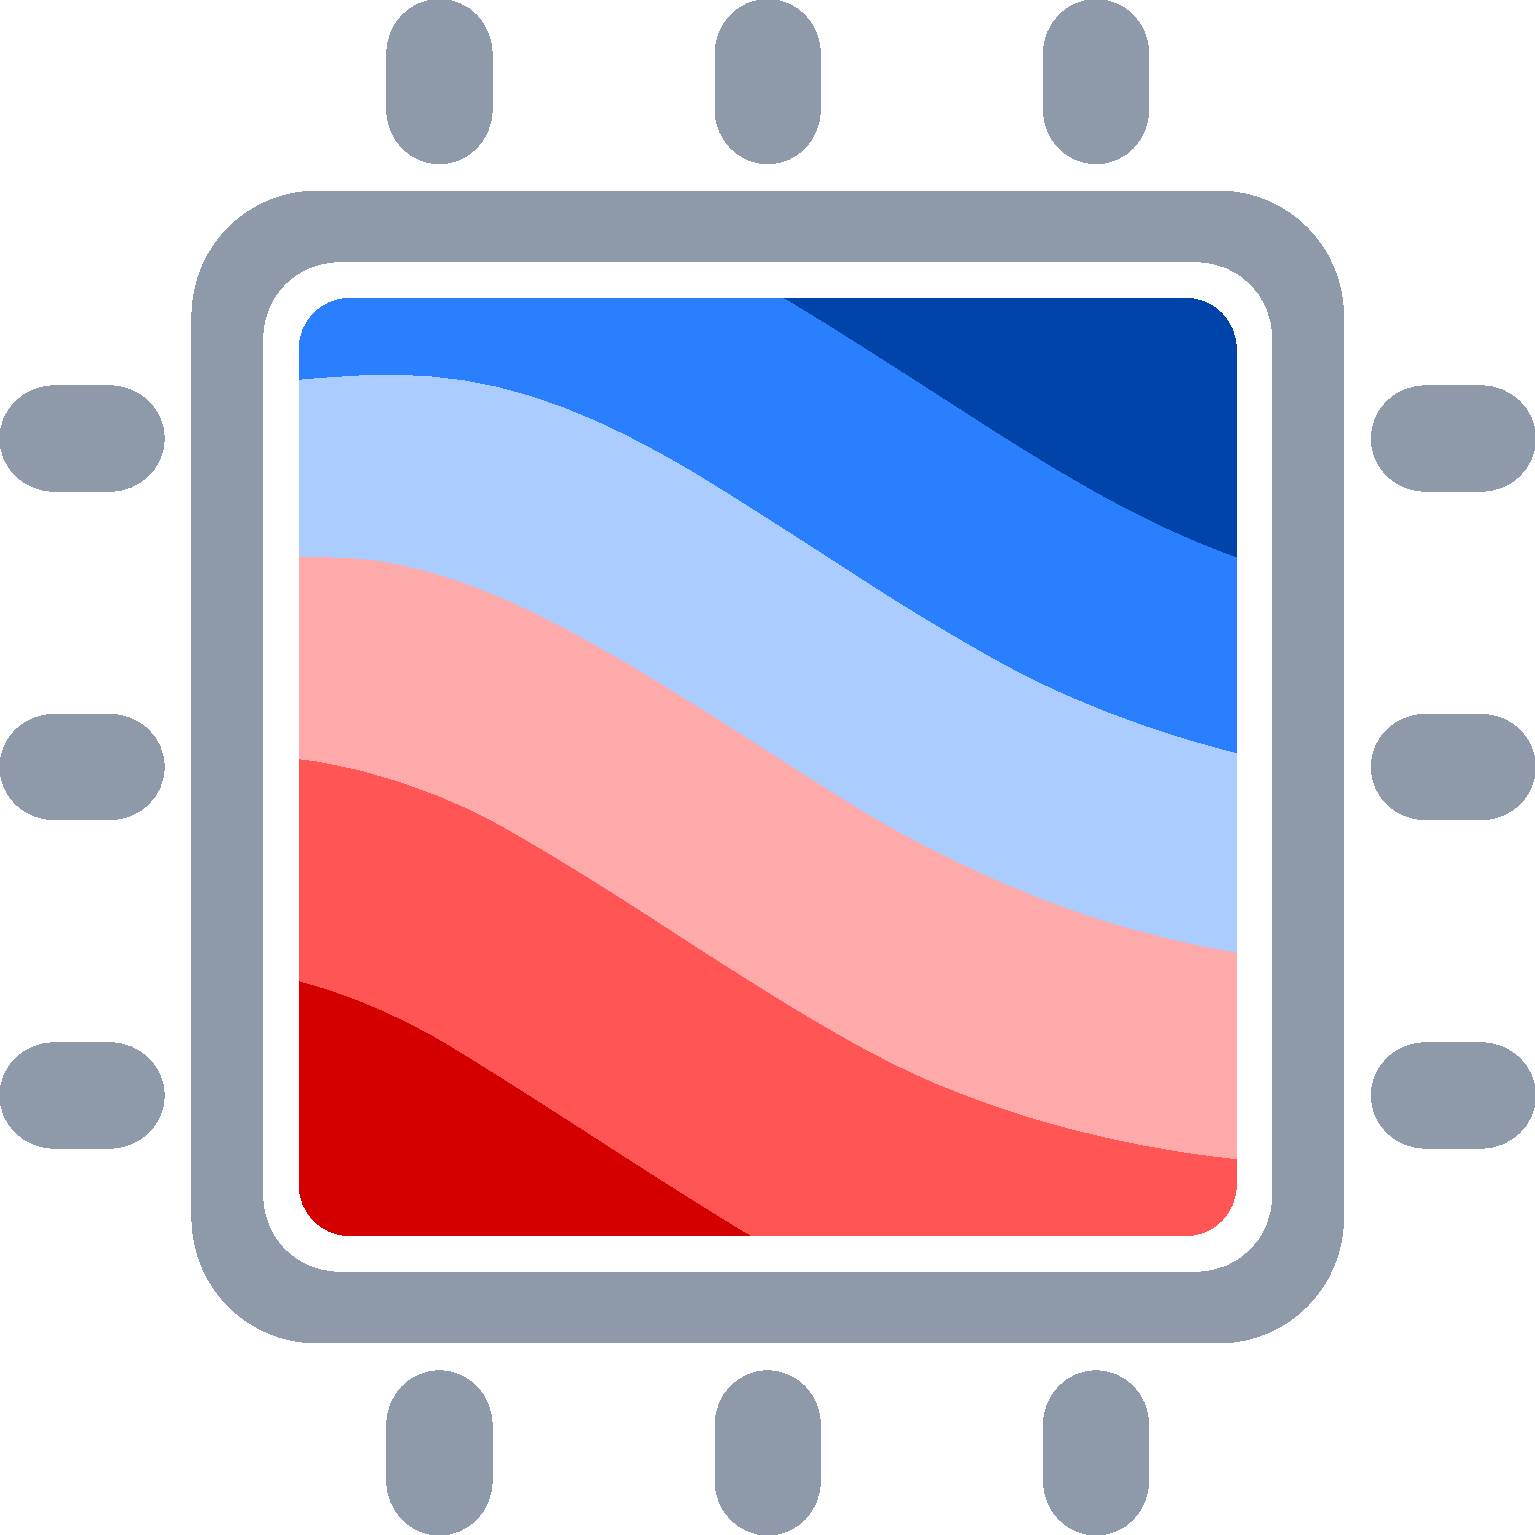
\includegraphics[height=2cm]{images/logo.pdf}
    \vspace{1cm}

    CONCURSO PÚBLICO

    PROFESSOR ADJUNTO A EM MLOPS

    INSTITUTO METROPOLE DIGITAL
    \vspace{5cm}

    \textbf{\LARGE MEMORIAL E PROJETO DE ATUAÇÂO PROFISSIONAL}
    \vspace{1cm}

    \textbf{\LARGE \MakeUppercase{\Author{}}}
    \vspace{5cm}

    {\small
      Apresentado para concurso público de títulos e provas para cargo de

      Professor Adjunto junto ao Instituto Metropole Digital

      Universidade Federal do Rio Grande do Norte.
      \vspace{1cm}

      Edital 069/2024-PROGESP
    }
    \vfill

    \Year{}
  \end{center}
\end{titlepage}

%==============================================================================
\chapter*{Resumo}

Possuo Bacharelado em Engenharia de Telecomunicações e Mestrado em Ciência da Computação pela \UFF{}.
Atualmente, estou cursando o Doutorado em Ciência da Computação na \UFRN{}.

Atuei como professor no programa PRONATEC e monitor da disciplina de Microprocessadores na \UFF{}. Desde a graduação,
venho me dedicando ao desenvolvimento e implementação de sistemas, com destaque para minha atuação no Laboratório de
Difração de Raios X da UFF (\textbf{LDRX}) durante uma bolsa do CNPq. Posteriormente, ampliei essa experiência em meu
estágio na GO2WEB e no desenvolvimento de sistemas de ensino a distância na UFF, além de meu trabalho atual na SEDIS-UFRN.
Essa trajetória também me proporcionou sólida expertise em extração e tratamento de dados.

Meu interesse em Inteligência Artificial começou na graduação, mas foi com o advento das LLMs que tive a oportunidade
de trabalhar mais intensamente com essa tecnologia, utilizando modelos abertos como o LLaMA~\cite{touvron2023llama}.
Minha atuação acadêmica inclui prêmios por trabalhos em Televisão Digital, com menções honrosas e publicações em eventos
relevantes.

Este memorial apresenta minha formação e trajetória profissional, incluindo reflexões sobre os fatores que me trouxeram
até aqui, as lições aprendidas ao longo do caminho e minha motivação para retornar à carreira acadêmica. Além disso, o
documento relata meus planos futuros para minha atuação no IMD e os projetos que pretendo desenvolver.



% usar linha do tempo?

%==============================================================================
\tableofcontents

\mainmatter
\pagestyle{fancy}

%==============================================================================
\chapter{Introdução}

\begin{summarybox}[frametitle=\faInfoCircle{}\quad Informações para contato]
  \begin{fa-ul}
    \faEnvelope & email: \href{mailto:\Email}{\Email} \\
    \aiLattes & Currículo Lattes: \url{https://lattes.cnpq.br/\Lattes} \\
    \faUser & Página pessoal: \url{https://esdrascaleb.github.io/} \\
    \aiOrcid & ORCID: \href{https://orcid.org/\ORCID}{\ORCID} \\
  \end{fa-ul}
\end{summarybox}

Ao longo da jornada acadêmica, acumulamos mais do que apenas certificados, diplomas e boas amizades.
Carregamos conosco o conhecimento e a experiência adquiridos, que permanecem como ferramentas valiosas, independentemente dos caminhos que seguimos.

Este documento tem como objetivo apresentar minhas atividades acadêmicas e profissionais,
com vistas à minha candidatura ao corpo docente do Instituto Metrópole Digital. As atividades estão organizadas em
tópicos que refletem as etapas da minha trajetória acadêmica e profissional, conectadas aos valores e motivações pessoais
que guiaram cada fase.

\section{Influências durante a infância e a adolescência}
Nasci e cresci em uma cidade de médio porte chamada Governador Valadares, em Minas Gerais. 
Meus pais se formaram em Engenharia Elétrica e desde criança tive contato com um computador 
inicialmente no trabalho do meu pai e em seguida em casa. Esse contexto sempre despertou em mim
uma paixão pela computação. Apesar de não usar computadores para programar sempre
tive curiosidade e configurava o computador para o tornar capaz de rodar os jogos que eu queria, mesmo quando o
hardware teoricamente não permitia.

Meu passatempo na escola no recreio costumava ser ler sobre as ultimas novidades
tecnologicas na biblioteca, a escola assinava as  revistas Galileu e Superinteressante que sempre traziam informações
interessantes e relevantes.

Quando tive acesso a internet me dediquei a aprender a utilizar os buscadores para encontrar 
a informação que eu gostava e me aprofundei em meus conhecimentos em implementação de sistemas
instalando e configurando emuladores para diversas plataformas em meu computador. Como não tinhamos
muito dinheiro eu podia jogar jogos antigos gratuitamente com o uso de emuladores.

Ao me mudar para o Rio de Janeiro tive aulas de programação na escola aprendendo Pascal e SQL. 
Até o vestibular tive muito interesse pela area de programação em especial para jogos chegando a 
fazer alguns projetos pequenos por conta própria e lendo sobre a área. Tentei vestibular para Engenharia da Computação
na UFRJ, mas passei mal em um dos dias de prova o que me custou uma nota ruim em química. Porem consegui ser aprovado
no vestibular da UFF para Engenharia de Telecomunicações, a escolha foi em inspiração ao meu pai que 
é Engenheiro de Telecomunicações na Oi desde a época que era Telebras.


\section{A estrutura deste memorial}

Este memorial está estruturado da seguinte forma. O capitulo~\ref{cap_uff} apresenta minha 
experiencia na graduação e mestrado na UFF. O capitulo~\ref{cap_atuacao} apresenta minhas atividades 
profissionais e académicas apos o mestrado. O capitulo~\ref{cap_pesquisa} apresenta minha pesquisa
atual e as razões de voltar a academia com o doutorado. O capitulo~\ref{cap_proje} apresenta
meus planos para o IMD e o IA360. E por fim o capitulo~\ref{cap_conclusao} apresenta minhas 
considerações finais.


%==============================================================================
\chapter{Formação Acadêmica na UFF}
\label{cap_uff}

\begin{summarybox}[frametitle=\faInfoCircle{}\quad Resumo da Formação acadêmica na UFF]
  \begin{datelist}
    \textbf{2005--2010} & \textbf{Bacharelado em Engenharia de Telecomunicações -- Universidade Federal Fluminense} \\
    2005-2006 & Voluntariado Laboratório de Computação da Engenharia - LACE \\
    2006 & Voluntário Pet-Tele \\
    2006 & Voluntariado Vestibular Solidário \\
    2006-2007 & Bolsita CNPQ no Laboratório de Difração de Raios X - LDRX \\
    2007-2008 & Bolsista Laboratório de AutoCad \\
    2008-2009 & Estágio na GO2WEB \\
    2010 & Registro do Software IPÚBLICA no qual tive Autoria \\
    2010 & Monitor da Disciplina de Microprocessadores \\
    2010 & Menção Honrosa com o Jogo DamsTV no WTVDI/WebMedia 2010 \\
    2010 & ShortPaper DamasTV no SBGames2010 \\
    2010 & Voluntário Brasil Game Show 2010 \\
    \textbf{2011--2013} & \textbf{Mestrado em Ciencia da Computação -- Universidade Federal Fluminense} \\
    2011 & Menção Honrosa com o Jogo DamsTV no 1º IPTV Application Challenge \\
    2011 & Voluntário Brasil Game Show 2011 \\
    2012 & Participação no Projeto Eduroam com a RNP \\
    2012 & Participação como Monitor do curso do Eduroam no 18º Seminário RNP de Capacitação e Inovação \\
    2012 & Participação como Monitor do curso do Eduroam no IdP Forum RNP \\
    2013 & Publicação do paper "JNS: An alternative authoring language for specifying NCL multimedia documents" no ICMEW 2013 \\
    2013 & Publicação do paper "NCL4WEB - Translating NCL Applications to HTML5 Web Pages no DocEng" 2013 \\
    2013 & Publicação no Software Registrado JNS Translator \\
    2013 & Participação no Software Registrado NCL4WEB \\
    2013 & Participação no Software Registrado JNS \\
  \end{datelist}
\end{summarybox}

Neste capitulo irei detalhar minha experiencia acadêmica durante a graduacao e mestrado. Minha 
atuação em pesquisa e extenção. Assim como os principais prémios e publicações.

\section{Graduação em Engenharia de Telecomunicação}
\label{sec_grad}
\begin{subsummarybox}[frametitle=\faGraduationCap{}\quad Bacharelado em Engenharia de Telecomunicações]
  \begin{fa-ul}
    \faUniversity & Universidade Federal Fluminense \\
    \faCalendar & Fevereiro 2005 -- Dezembro 2010 \\
    \faUser & Orientadora: Debora Muchaluat-Saade\\
    \faInfoCircle & DamasTV: um Jogo de Damas para o SBTVD	Accepted~\cite{saad2010damastv}
  \end{fa-ul}
\end{subsummarybox}
Desde o primeiro ano da graduação, eu procurava formas de acesso a uma bolsa de pesquisa, 
por isso, no segundo período  me tornei voluntário do laboratório de informática, 
objetivando me tornar efetivo no período seguinte quando reabrisse a seleção. 

No periodo seguinte tentei a seleção para o PET-Tele, mas acabei sendo rejeitado.
Porem ingressei no grupo como vuluntário e participei de cursos e ajudei na organização
do encontro regional de PET na UFF em 2006. No PET Tele, consegui participar da 
 Semana de Engenharia da Computação e Eletrônica da UFRJ. Neste evento aprendi um pouco sobre IA 
 e fiquei instigado a tentar a docencia o que me fez lecionar alguns meses no pré-vestibular
 comunitário da UFF.

No mesmo periodo, ingressei no Laboratório de 
Difração de Raios-X, pertencente ao Instituto de Física da UFF.
como bolsista do CNPQ. Minha experiência com a iniciação científica na Instituto de Física foi 
muito instrutiva, orientado pelo professor Carlos Basilio(hoje da UFMG). Aprendi sobre o tratamento 
de dados e desenvolvi uma aplicação para auxiliar a seleção de outliers de forma visual. Também 
tive contato com o software livre e a implementação de sistemas, auxiliando a implementação da rede 
interna do laborátório e a configuração de softwares para acesso remoto. 

Durante quase todos os anos da graduação participei das semanas academicas promovidas na engenharia,
frequentemente indo na semana de engenharia para conhecer novidades e pesquisas. Como fazia na escola, 
mas agora ao invés de ler revistas eu estava indo ver pessoalmente.

Apos o fim da pesquisa no LDRX, 5º período, eu me tornei monitor do laboratório de Autocad[3] 
onde aprendi mais sobre o sistema Linux. Neste contexto acadêmico, fui integrante da liderança de um  
movimento estudantil na Universidade: o Alfa e Ômega (o qual já era membro desde meu 3º período), 
uma experiência durante toda a graduação na qual aprendi:  formas de articulação para falar em público, 
a trabalhar com gestão de pessoas e a conhecer métodos de liderança, pois o grupo oferecia cursos e treinamentos práticos.  
Com o grupo tive também experiencias para treinar meu ingles sendo parte de voluntários no PanAmericano pela
Organização More Than Gold.

No meu 7º período, comecei a procurar por estágio, sendo assim, em 2008, fui aprovado em um estágio 
que durou 1 ano e meio na Go2Web, uma empresa de desenvolvimento de sistemas web. Nessa
empresa aprendi a programar no paradigma orientado a objetos com C\# e a o framwork .NET bem como 
programação Web com ASP, HTML JavaScript e CSS.
Dentre as mais notáveis conquistas pessoais e profissionais nesta empresa, pode-se destacar o 
desenvolvimento de um software para gestão governamental o IPUBLICA~\cite{ipu_sistema_gestao}.
No qual eu utilizei a biblioteca do gogolemaps para criar um dashboard de gestão para a prefeitura 
do Rio de Janeiro.

No ano de 2009, eu fiz uma disciplina optativa com a minha futura orientadora a professora 
Débora Christina Muchaluat Saad, a disciplina era multimídia e televisão digital. Na qual,
meu trabalho de conclusão da disciplina foi a primeira versão do DamasTV, um jogo para o middleware 
interativo Ginga-NCL~\cite{soares2007ginga} do sistema brasileiro de televisão digital~\cite{mendes2007sbtvd}. 
O jogo foi feito em Lua e posteriormente foi evoluido para funcionar pelo canal de retorno da televisão
possibilitando jogar com pessoas pela internet.
Atravez desse trabalho eu ingressei no grupo de pesquisa Midiacom e enviei meu primeiro trabalho academico,
que foi regeitado pelo SBGames2009.

Em 2010 fui monitor da disciplina de Microprocessadores,  minha segunda experiência 
relacionada a docência. Eu havia adquirido mais habilidade para falar em público, através da minha 
participação em movimento estudantil. Dessa forma,  tive uma boa experiência ao aplicar aulas de 
laboratório e reposição para a turma. Fiquei motivado com a área de ensino, pois senti prazer e 
felicidade ao ver as pessoas evoluindo o conhecimento com o meu auxilio. 

Ainda em 2010, meu aritgo~\cite{saad2010damastv} sobre o DamasTV, foi aprovado para o SBGames 2010, foi 
apenas um ShortPaper. Porém, este shortpaper me permitiu ir ao SBGames. O SBGames2010 não foi a 
maior conferência que já fui, mas sem dúvida foi a que mais gostei, aprendi sobre jogos Educativos 
feitos para realmente serem jogos e não um mero Quiz eletrônico. Aprendi sobre desenvolvimento de 
grandes jogos com o exemplo o Taikodom da Hoplon. Conheci o mercado Brasileiro de games e empresas 
que estavam se aventurando nela, como a MiniBoss e a Vortex.

Neste mesmo ano o jogo que desenvolvi, DamasTV, ganhou seu primeiro prêmio internacional: uma menção 
honrosa no 1º Concurso Latino Americano de aplicação para televisão digital, que aconteceu no Workshop 
de Televisão Digital no WebMidia 2010.

No segundo semestre de 2010, participei da disciplina de programação gráfica e jogos digitais com o 
professor Esteban Clua. Foi a disciplina mais divertida que fiz, meus trabalhos por vezes eram 
programar jogos e fui aprovado com excelência. No trabalho final da disciplina, construí um 
protótipo de um engine de jogos para televisão digital, com base no trabalho de Diego Bastos o 
GingaGame~\cite{barboza2009ginga}, que era em Java. Eu criei um prototipo do GingaGameNCLua 
que era em NCLua.

Mediante a convivência com o professor Esteban, fui convidado a participar do Festival 
“Brasil Game Show” de 2010, nas funções de organizador e colaborador. Auxiliando a 
organização e execução da Brasil Game Jam, das palestras e do concurso de jogos. 

Ao fim daquele ano defendi meu trabalho de conclusão de curso, o DamasTV: um Jogo Interativo para 
Televisão Digital. Na minha banca estiveram as professoras Maria Luíza (coordenadora do meu curso 
e professora da matéria de programação orientada a objetos), o professor Esteban Clua e a 
professora Débora Saad, minha orientadora. Fui aprovado com nota máxima e decidi fazer o 
mestrado com minha orientadora que havia saído do departamento de Engenharia de Telecomunicações 
e entrado no deparamento de Ciência da Computação. Dessa forma pude ir para área que era minha intenção
no vestibular.


\section{Mestrado em Ciência da Computação}
\label{sec_mes}
\begin{subsummarybox}[frametitle=\faGraduationCap{}\quad Mestrado em Ciência da Computação]
  \begin{fa-ul}
    \faUniversity & Universidade Federal Fluminense \\
    \faCalendar & Fevereiro 2011 -- Junho 2013 \\
    \faUser & Orientadora: Debora Muchaluat-Saade\\
    \faInfoCircle & JNS E NCL4WEB: AUXILIANDO O DESENVOLVIMENTO E DIVULGAÇÃO DE DOCUMENTOS NCL~\cite{silva2013jns}
  \end{fa-ul}
\end{subsummarybox}
O mestrado começou logo após a graduação, eu tinha como orientadora, Debora Christina Muchaluat Saade, a professora com quem fiz o trabalho de conclusão de curso. Embora meu desejo fosse iniciar um projeto na área de games com o professor Esteban Clua, decidi seguir o mestrado com a minha orientadora na linha de pesquisa de sistemas de multimídia e televisão digital. Pois além de ser uma área promissora, eu percebi que ainda deveria contribuir a pesquisa nesta área em tópicos ainda não explorados. Pois meu projeto com o professor Estevan séria uma engine para jogos de televisão digital, algo que já estava sendo desenvolvida pela UFPB a mais de um ano.
 Desde o primeiro período fui direcionado para na minha dissertação, trabalhar com algumas opções: terminar minha engine, trabalhar com a linguagem de Templates XTemplate 3.0[11] ou criar uma nova alternativa de linguagem com um script. Por perceber que a linguagem NCL era muito complexa para quem estava acostumado à programação procedural, preferi desenvolver uma linguagem à fazer uma engine de jogos. Pois, na época, existia outro grupo já desenvolvendo uma engine para NCLua na UFPB, e eu não queria trabalhar com algo que já estava sendo feito.
Iniciei meu projeto cujo foco era desenvolver uma espécie de script para a linguagem de marcação NCL usada na televisão digital. Estudei a fundo as linguagens multimídia existentes: SMIL[12], NCL, MHEG[13] e a linguagem proposta no padrão japonês o BML[14]. Constatou-se que com exceção de uma do padrão europeu MHEG, todas eram baseadas em XML[15], dessa forma, como o XML estava sendo substituído pelo JSON[16] no meio WEB[17], resolvi então, criar uma linguagem com base no JSON.  Nas disciplinas de 2011 desenvolvi quatro artigos:

Em 2011, eu participaria de novo da Brasil Game Show como Staff, porém a conferência seria reduzida 
a pequenos Keynotes com palestrantes mais famosos, como  Zafer Coban um dos produtores do Bataman 
Arkan City, da Warner Games e o Yroshinori Ono, produtor do Street Fighter 4 da Capcom.

I.  Um survey sobre jogos e redes P2P[18] para a disciplina de redes de computadores do mestrado. No artigo fiz um survey sobre como os jogos MMO usam rede P2P, citando as vantagens e desvantagens do uso da mesma, além de citar as principais pesquisas[19] e avanços sobre o tema.
II. Um artigo sobre uso de GPUs[20] para simulações, onde utilizei uma GPU para gerar números aleatórios. Como as GPUs usam processamento paralelo em vários núcleos, obtive uma velocidade 50% mais rápida usando as mesmas do que usando somente o computador.
III. Um artigo sobre internet do futuro, em que discorri sobre um dos testbeds[21] (grandes centros centro de teste de protocolos de rede) da Europa: o Geni[22] e uma interface que estende o uso mesmo o ProtoGeni[23]. Esta usa a API do Geni para o interligar os seus clusters com o EmuLab[24],  criando uma infra-estrutura gigante para testes de novos protocolos para internet (testbed).
IV. E por fim, um artigo sobre como documentar documentos em JSON, discutindo sobre o funcionamento do JSON-Schema[25].

Todos os artigos produzidos nestes períodos não chegaram a ser aceitos para nenhum congresso, mas me ajudaram a amadurecer na maneira de produzir artigos. Ainda em 2011, destacamos algumas importantes realizações:

I. Participei da Brasil Game Show2011, como coordenador dos monitores da Game Jam dos keynotes e da pré-organização do Festival de Jogos.
II. O DamasTV ganhou o seu segundo prêmio internacional: uma menção honrosa no IPTV Challenge 2011 do ITU.
III. Apresentei uma palestra sobre o desenvolvimento de jogos para televisão digital no 2º Seminário de Simulação do SENAI-RJ.

A partir de 2012, fiz parte do projeto Eduroam[26], projeto que liga todo o mundo através de unidades federadas em universidades para promover acesso sem fio seguro. Auxiliei a implementação da rede Eduroam na Universidade Federal Fluminense (UFF). Além de participar como monitor de três cursos sobre o sistema Eduroam para Escola Superior de Redes da Rede Nacional de Ensino e Pesquisa (RNP). Dentre os cursos: um na escola técnica de redes no Rio de Janeiro, um no fórum RNP em Brasília e um no Seminário RNP de Capacitação e Inovação em Foz do Iguaçu.
Durante todo o mestrado estive também envolvido no grupo de pesquisa em Televisão Digital no Laboratório Midiacom, da Universidade Federal Fluminense.  Em relação a minha dissertação, inicialmente, minha linguagem de script o JNS (JSON NCL Script) estava completa e eu estava terminando de desenvolver o tradutor/compilador da mesma para NCL. Mas, após apresentá-la na reunião do grupo de pequisa, me foi sugerido que esta fosse capaz de ser traduzida em outras linguagens multimídia além do NCL. Minha orientadora sugeriu que fizessémos a tradução para o HTML5[27]. Esta contribuição me levou, ao invés de fazer algo restrito a minha linguagem, à desenvolver um sistema que traduzisse a linguagem NCL para o HTML5. Assim, os desenvolvedores de NCL teriam maior facilidade para publicar o seu trabalho. E a minha linguagem poderia ser traduzida para HTML5, como a mesma era compilada para NCL.
Diante deste caminho, e com o conhecimento adquirido nas disciplinas do mestrado, criei o NCL4WEB:  uma ferramenta que usava o XSLT e o JavaScript para transformar automaticamente um código NCL em um código em HTML5. Desta forma, poderíamos traduzir de JNS para NCL e do NCL para HTML5. A idéia por traz disso era permitir ao desenvolvedor NCL publicar o seu trabalho na WEB sem requerer dele nenhum conhecimento de HTML.

Nessa perspectiva, enviei um artigo sobre o JNS para o congresso WebMedia 2012, porém, o mesmo não foi muito aceito, pois parecia que eu estava querendo substituir a linguagem NCL, mesmo não indo ao WebMedia de 2012 (principal conferência brasileira sobre multimídia), o lançamento do NCL4WEB pela internet gerou grande repercussão no congresso.
No final do meu segundo ano no mestrado, consegui publicar um artigo sobre o NCL4WEB no DocEng 2013[28] (Qualis B1 capes) e um artigo sobre o JNS para o workshop de gerenciamento  de informação em multimídia e indústria (MIS-MEDIA 2013) do ICME 2013[29] (quális A1 capes). Tive que pedir um tempo maior para concluir minha dissertação de mestrado, pois esta havia ficado muito grande e eu tinha que avaliar os testes feitos com os usuários sobre a linguagem JNS.
Para minha banca de mestrado tive a minha orientadora Débora Christina Muchaluat Saad, Vanessa Braganholo também professora da UFF (quem me apresentou ao XSLT[30]) e professor Marcelo Ferreira Moreno, da Universidade Fedral de Juíz de Fora (outras das pessoas que ajudou e ainda ajuda o desenvolvimento da linguagem NCL). Em agosto de 2013 defendi minha dissertação de mestrado: “JNS e NCL4WEB: Auxiliando o Desenvolvimento e Divulgação de Documentos NCL”.


%==============================================================================
\chapter{Atuação Profissional apos Mestrado}
\label{cap_atuacao}

\begin{summarybox}[frametitle=\faInfoCircle{}\quad Resumo da Atuação Profissional]
  \begin{datelist}
    2013 & Professor do Curso de Cabeamento Estruturado no IFRN Parnamirim pelo PRONATEC \\
    2014-2015 & Atuação como Desenvolvedor Moodle na SEDIS pela FUNPEC \\
    2015 & Participação da organização do capitulo local da Global Game Jam \\
    2015-atual  & Técnico de TI - Servidor Federal da UFRN \\
    2015-2020 & Participação no Projeto AVASUS \\
    2023 & Participação do projeto Piloto a Capes para Monitoramento do Ensino a Distáncia \\
  \end{datelist}
\end{summarybox}



Meu intuito após o mestrado era fazer o doutorado. No entanto, por pretender me casar antes disso, por razões pessoais me mudei para a cidade de Natal/RN, após ser aprovado em processos seletivos para professor, e posteriormente para programador de jogos.


Experiência Docente

Em minha graduação na UFF participei do vestibular solidário por alguns meses e fui monitor da disciplina de microprocessadores por 2 semestres. Ministrei alguns mini cursos na RNP sobre a rede Eduroam enquanto estive no mestrado e era bolsista do laboratório Midiacom.
Em Natal, em 2013, fui aprovado em um processo seletivo para professor do Programa Nacional de acesso ao Ensino Técnico e Emprego (PRONATEC) no Instituto Federal de Educação, Ciência e Tecnologia do Rio Grande do Norte, (IFRN), de Parnamirim, onde ministrei duas disciplinas:  Cabeamento estruturado e Redes de Acesso; e Planejamento e Projeto de Redes de Computadores.
Apos me tornar servidor da SEDIS em 2015, ministrei alguns cursos sobre o uso básico e avançado do sistema de ensino a distáncia Moodle, do qual sou especialista.


4.2      Experiência Técnica e Científica

No final de 2013, fui aprovado em uma seleção da FUNPEC, para atuar na SECRETARIA DE EDUCAÇÃO A DISTANCIA (SEDIS) na função de programador de jogos. Em 2014 fui convocado, e desde o presente momento, venho desenvolvendo atividades referentes ao desenvolvimento de sistemas e aplicações, determinando interface gráfica, critérios ergonômicos de navegação, montagem de estrutura de banco de dados e codificação de programas; responsável por projetar, implantar e realizar manutenção de sistemas e aplicações; selecionando recursos de trabalho, tais como metodologias de desenvolvimento de sistema, linguagem de programação e ferramentas de desenvolvimento.
Além do planejamento de etapas e ações de trabalho, executei projetos ligados a área de ensino a distância, como sistemas que se integram ao Moodle Acadêmico[31] e sistemas ligados a área de telesaude, como um aplicativo de diagnóstico interativo em HTML5.
Em 2015 fui aprovado para o cargo de técnico de TI na UFRN, continuei na Secretária de Educação a Distância me Focando por 8 anos na evolução e manutenção do projeto de ensino a distância continuada para o SUS o Avasus. Neste tempo auxiliei a extração de dados dos sistemas de ensino a distância para criação de pesquisas academicas, fui creditado em algumas delas [34].
Apos a pandemia passei a reavaliar a minha vida e decisões e decidi tentar novamente me tornar um docente, iniciando o doutorado junto a Programa De Pós-Graduação Em Sistemas E Computação Administração (PPgSC). Desde então tenho voltado a escrever diretamente artigos para conferencias. Tendo me dedicado mais a pesquisa em modelos de IA criando aplicações para tarefas academicas com modelos de IA, como uma aplicação usando o BERT para a qualificação de artigos com python e criando uma implementação com modelos quantificados para a mesma aplicação na web: https://esdrascaleb.github.io/websm/.
Espero continuar essa jornada junto a UFRN como docente e usar meus conhecimentos antigos e novos para promover o conhecimento e bem estar da sociedade.




%==============================================================================
\chapter{Pesquisa Atual no Doutorado}
\label{cap_pesquisa}


\section{Atividades de Extensão}




\chapter{Projeto de Atuação Profissional}
\label{cap_proje}

Além de ministrar aulas, pretendo desenvolver projetos com IA para auxiliar startups e empresas júnior da cidade na
implementação de modelos generativos em seus serviços e produtos. O objetivo é ensinar estratégias para o uso de IAs
quantizadas e de baixo custo operacional, permitindo a implementação diretamente no cliente e, assim, reduzindo os
custos para as startups em especial as empresas do Parque Tecnológico do IMD.

Também planejo iniciar projetos pilotos para o uso de IA em diversas áreas, tais como:
Inclusão Digital para Idosos: Ajudar idosos a navegar no ambiente digital com segurança atravez de cursos voltados ao uso de assistentes virtuais. Reduzindo sua vulnerabilidade a informações falsas e promovendo sua inclusão digital.
Tutoria Virtual para Estudantes: Implementar pipilenes de modelos para serem tutores virtuais para dar suporte personalizado aos alunos em disciplinas específicas, ajudando a melhorar o desempenho acadêmico e a reduzir a carga de trabalho dos professores.
Secretários Virtuais Acadêmicos: Desenvolver secretários virtuais para simplificar processos acadêmicos, facilitando a vida dos alunos e aumentando a eficiência no trabalho dos servidores.
Gestão Inteligente de Energia e Resíduos: Implementar modelos inteligentes para otimizar o uso de energia no campus, alertando para luzes ou ar-condicionado deixados ligados em salas, e para uma coleta de lixo eficiente, com notificações automáticas para agilizar o recolhimento.
Apoio a acessibiliade: Auxiliar  o desenvolvimento soluções que auxiliem a acessibilidade como cães guias virtuais para pessoas com deficiencia visual, leitores de libras mais avançados para deficientes auditivos e assistentes para pessoas com dificuldade de socialização.


%==============================================================================
\chapter{Conclusão}
\label{cap_conclusao}

Minha trajetória acadêmica e profissional é marcada pela busca constante por aprendizado, inovação e contribuição à
sociedade por meio da tecnologia. Cada etapa, desde meus primeiros projetos na graduação até os desafios atuais no
doutorado, moldou minhas competências e consolidou minha paixão pela docência e pela pesquisa aplicada.

Minha motivação para atuar no IMD está diretamente ligada ao potencial de impactar positivamente a formação de
profissionais e à oportunidade de desenvolver soluções práticas para desafios reais. Acredito que minha experiência
em áreas como sistemas interativos, ensino a distância e inteligência artificial, combinada com meu comprometimento
com a inclusão digital e acessibilidade, me permitirá agregar valor ao Instituto e contribuir para o sucesso de
iniciativas como o IA360.

Estou determinado a continuar expandindo o conhecimento e promovendo inovações que transcendam a academia, criando um
impacto duradouro na indústria, na sociedade e no ambiente educacional. Este memorial reflete não apenas o percurso
que me trouxe até aqui, mas também minha visão de futuro e o desejo de construir um legado de transformação e excelência.



%==============================================================================
\backmatter
\bibliographystyle{apalike-doi}
\bibliography{references}

\end{document}
